\section{Implementation}\label{sec:implementation}

In this section we describe an implementation of a SQL compiler and
runtime based on \dbsp.

\subsection{The \dbsp Rust runtime}\label{sec:runtime}

We have built an implementation of \dbsp as part of an
open-source~\cite{dbsp-repo} project with an MIT
license~\cite{dbsp-crate}.  The implementation consists of a Rust
library for building circuits and a runtime that executes these
circuits using a pool of worker threads.

The library provides APIs for basic algebraic data types: such as
groups, finite maps, \zrs, indexed \zrs.  The core data structure of
the library for representing processed data is the ``time-indexed,
indexed \zr''.  This is the most general data structure needed in
recursive circuits.  It represents a vector (indexed by time) of
indexed \zrs.  Simple indexed \zrs are represented by a vector with a
single element, while \zrs are represented as indexed \zrs with an
empty value.\footnote{Rust is very efficient at eliding empty data
structures.}  The starting point of this implementation was the
differential dataflow trace data structure~\cite{dd-crate}.

A circuit construction API allows users to create \dbsp circuits by
inserting operator nodes --- boxes in our diagrams --- and connecting
them with streams --- the arrows in our diagrams.  The library
provides more than 70 pre-built generic operators for integration,
differentiation, delay, nested integration and differentiation, and
basic \zr incremental operators, corresponding to plus, negation,
grouping, joining, semi-joins, anti-joins, temporal joins, primitive
aggregates, generic aggregates (fold), $\distinct$, flatmap, window
aggregates, indexing, upsert, etc.  Some operators only exist in a
pure incremental form (e.g., they only operate correctly when fed
deltas), and thus, when used in a non-incremental circuit, have to be
``inverted'' using the inversion property from
Proposition~\ref{prop-inc-properties}.

For iterative computations the library provides the $\delta$ operator
and an operator that generalizes $\int$ by terminating iteration when
\emph{all} the operators in the corresponding circuit cycle have
reached a fixed point, which is detected when neither outputs or state
change in an execution step.  The low level library allows users to
construct incremental circuits manually by stitching together
incremental and non-incremental versions of primitive operators.

The library also provides many ``helper'' operators that are used by
the code generator in the implementation of some streaming queries,
e.g., for state garbage-collection (a subject not discussed in this
paper).

\subsubsection{Parallelization and Scale-out}

Besides computing on streams, \dbsp circuits look very much like other
dataflow query engines.  As such, all standard parallelization
algorithms described in the literature~\cite{Graefe-sigmod90} can be
applied.  Our core circuits library automatically parallelizes each
circuit by sharding each operators to execute using a specified number
of worker threads (all operators use the same number of threads, which
is statically-defined).  The library automatically inserts exchange
operators to re-shard data when necessary (e.g., shard on the common
key in an equi-join).  The same scheme can be used to implement
scale-out solutions across multiple machines, but this part of the
runtime is still under development.

\subsubsection{State management}\label{sec:state-management}

Incremental computation is not free.  It is in fact a trade-off
between time and space.  While many incremental query primitives are
``stateless'', some important classes of database operations,
including joins, $\distinct$, and group-by-aggregate use $\I$
operators in their incremental expansion.  This state is kept in
\emph{indexes}.  (In the \dbsp theoretical model the state is stored
in delay operators $\zm$ and $\lift{\zm}$, but these are always inside
integrators $\I$.)  All other operators are stateless.

The size of these indexes is proportional to the size of the total
input data of these operators --- and thus the total state of a
circuit can even exceed the size of the original database.  (Many
traditional IVM schemes opt to recompute this state on demand, rather
than store it permanently; \dbsp can model this strategy.)

At runtime, linear operators are essentially free.  The performance of
a \dbsp program is given by the cost of maintaining and
accessing the indexes.

Indexes provide two essential operations:
\begin{description}
\item[Write:] Merging an existing (large) index with a new (small) change.
\item[Read:] Looking up a (small) set of values.
\end{description}

Our implementation of indexes performs both these operations in
amortized time $O(k \log n)$, where $k$ is the size of the changes,
and $n$ is the size of the index.  The implementation of indexes is
essentially a Log-Structured Merge (LSM) Tree~\cite{oneil-ai96}.

The data structure used for indexes, (called a \emph{trace} in the
code), is shown in Figure~\ref{fig:trace}.  Each index is represented
as a sequence of sorted immutable lists (called \emph{batches}), of
exponentially increasing sizes (1, 2, 4, 8, etc.) --- a generalization
of binary signed digits~\cite{signed-digits}.  Any batch is sorted
lexicographically, first on the index, then on the value.  Each batch
is a \zr, and a trace represents the \zr that is the sum of all
component batches.  The same tuple can appear in different batches
with different weights, but appears at most once in each batch.  Since
addition is commutative and associative, parts can be added in any
order.

\begin{figure}[h]
  \begin{center}
    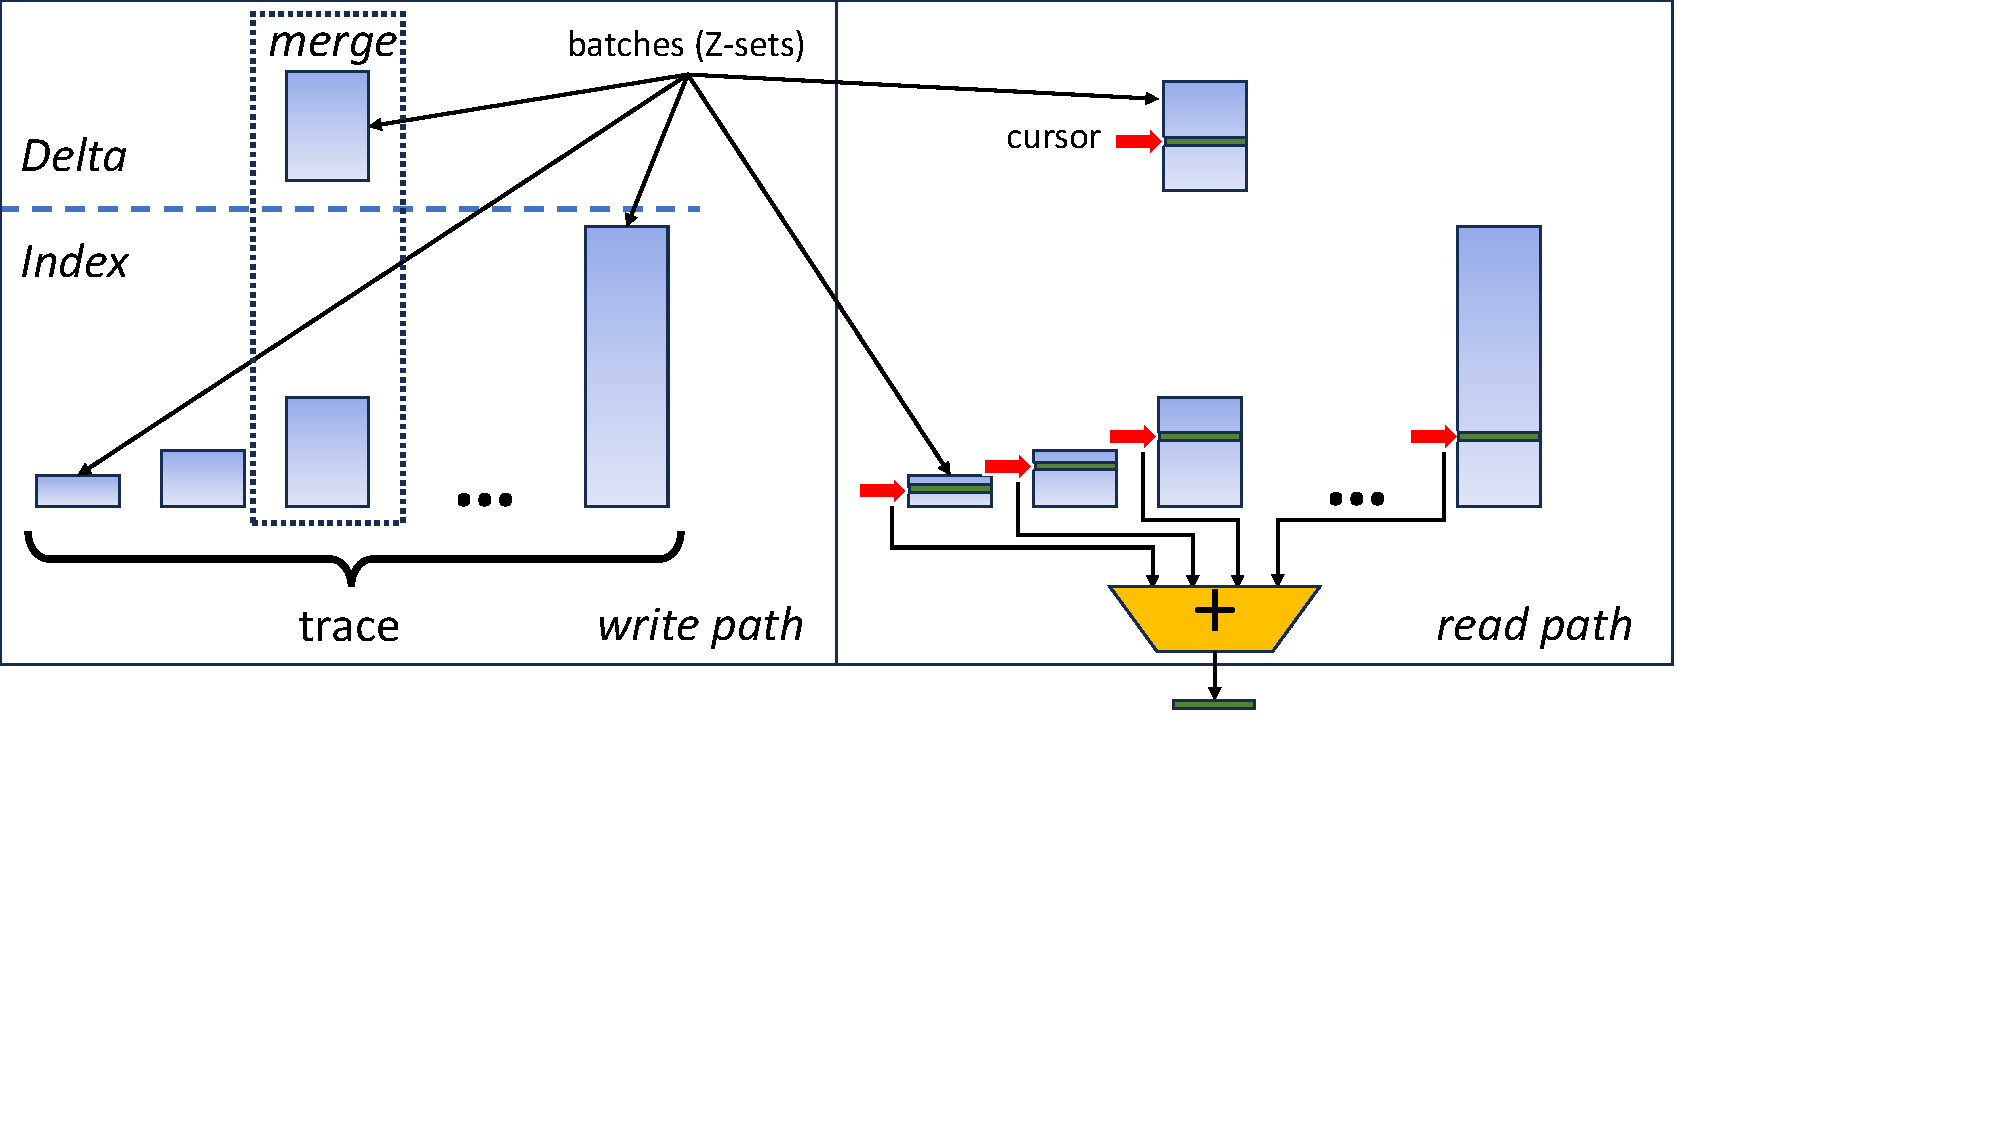
\includegraphics[trim={0 2.9in 2.1in 0},clip,scale=.27]{trace.pdf}
    \caption{\label{fig:trace}Index representation and access.}
  \end{center}
\end{figure}

A change added to an index is represented as a single batch, sorted
using the same order as the index.  When the index ingests a new
change (left side of Figure~\ref{fig:trace}), the new batch is simply
appended.  As the index grows, batches of similar size are lazily
merged.  Merges are performed by background compaction threads; each
merge may span multiple circuit steps.  The result of merging 2
batches with \(n_1\) and \(n_2\) tuples has \(n_1 + n_2\) or fewer
tuples, and can even be empty if all weights add to 0.

Exponential search~\cite{bentley-ipl76} is used to lookup the tuples
of a change inside an index (right side of Figure~\ref{fig:trace}) .
When the same tuple is found in multiple lists, the corresponding
weights are added.

\subsection{Secondary storage}

Since indexes can be very large, in many applications they need to be
spilled to disk.  Persistent storage also helps for fault tolerance.

Initially we considered reusing an existing storage engine for
persisting state.  Using RocksDB~\cite{dong-ats21} seemed a great
choice due to its architectural similarities to the way we manage state
in-memory.  RocksDB is mature, widely used, and well-maintained
software.

RocksDB is a generic key-value store that can represent multiple
indexes using its column family feature, with distinct namespaces for
keys. It also offers all the APIs we needed: quick value retrieval for
a given key and iteration over keys and values (both forward and
backward) from a starting point.  RocksDB is also based on an
LSM-Tree.

The mature RocksDB Rust library provides all need\-ed operations,
including custom comparators for keys, zero-copy get operations, bulk
inserts, and control over merging of entries with the same key during
compaction.

Integrating RocksDB into our system was straightforward.  We
implemented the trace API described in the previous section.
Unfortunately, we encountered several critical issues:

\paragraph{Lack of Scaling.} Our implementation utilizes multiple threads
effectively by sharding data, allowing the system to scale well across
many CPUs.  To avoid contention, we placed each persistent index in a
separate column family in RocksDB. However, we discovered that RocksDB
doesn't scale well beyond a few threads. In fact, with RocksDB, our
pipelines performed best with a single thread.

Figure~\ref{fig:rocksdb} illustrates the severity of the issue (note
the log-scale on the y-axis). It shows the performance for a subset of
the Nexmark queries that use indexes, comparing RocksDB with a single
thread against RocksDB with eight threads. For reference, we also
include the performance of our system configured to keep everything in
DRAM data structures (which, as expected, performs much better).

\begin{figure}[h]
  \begin{center}
  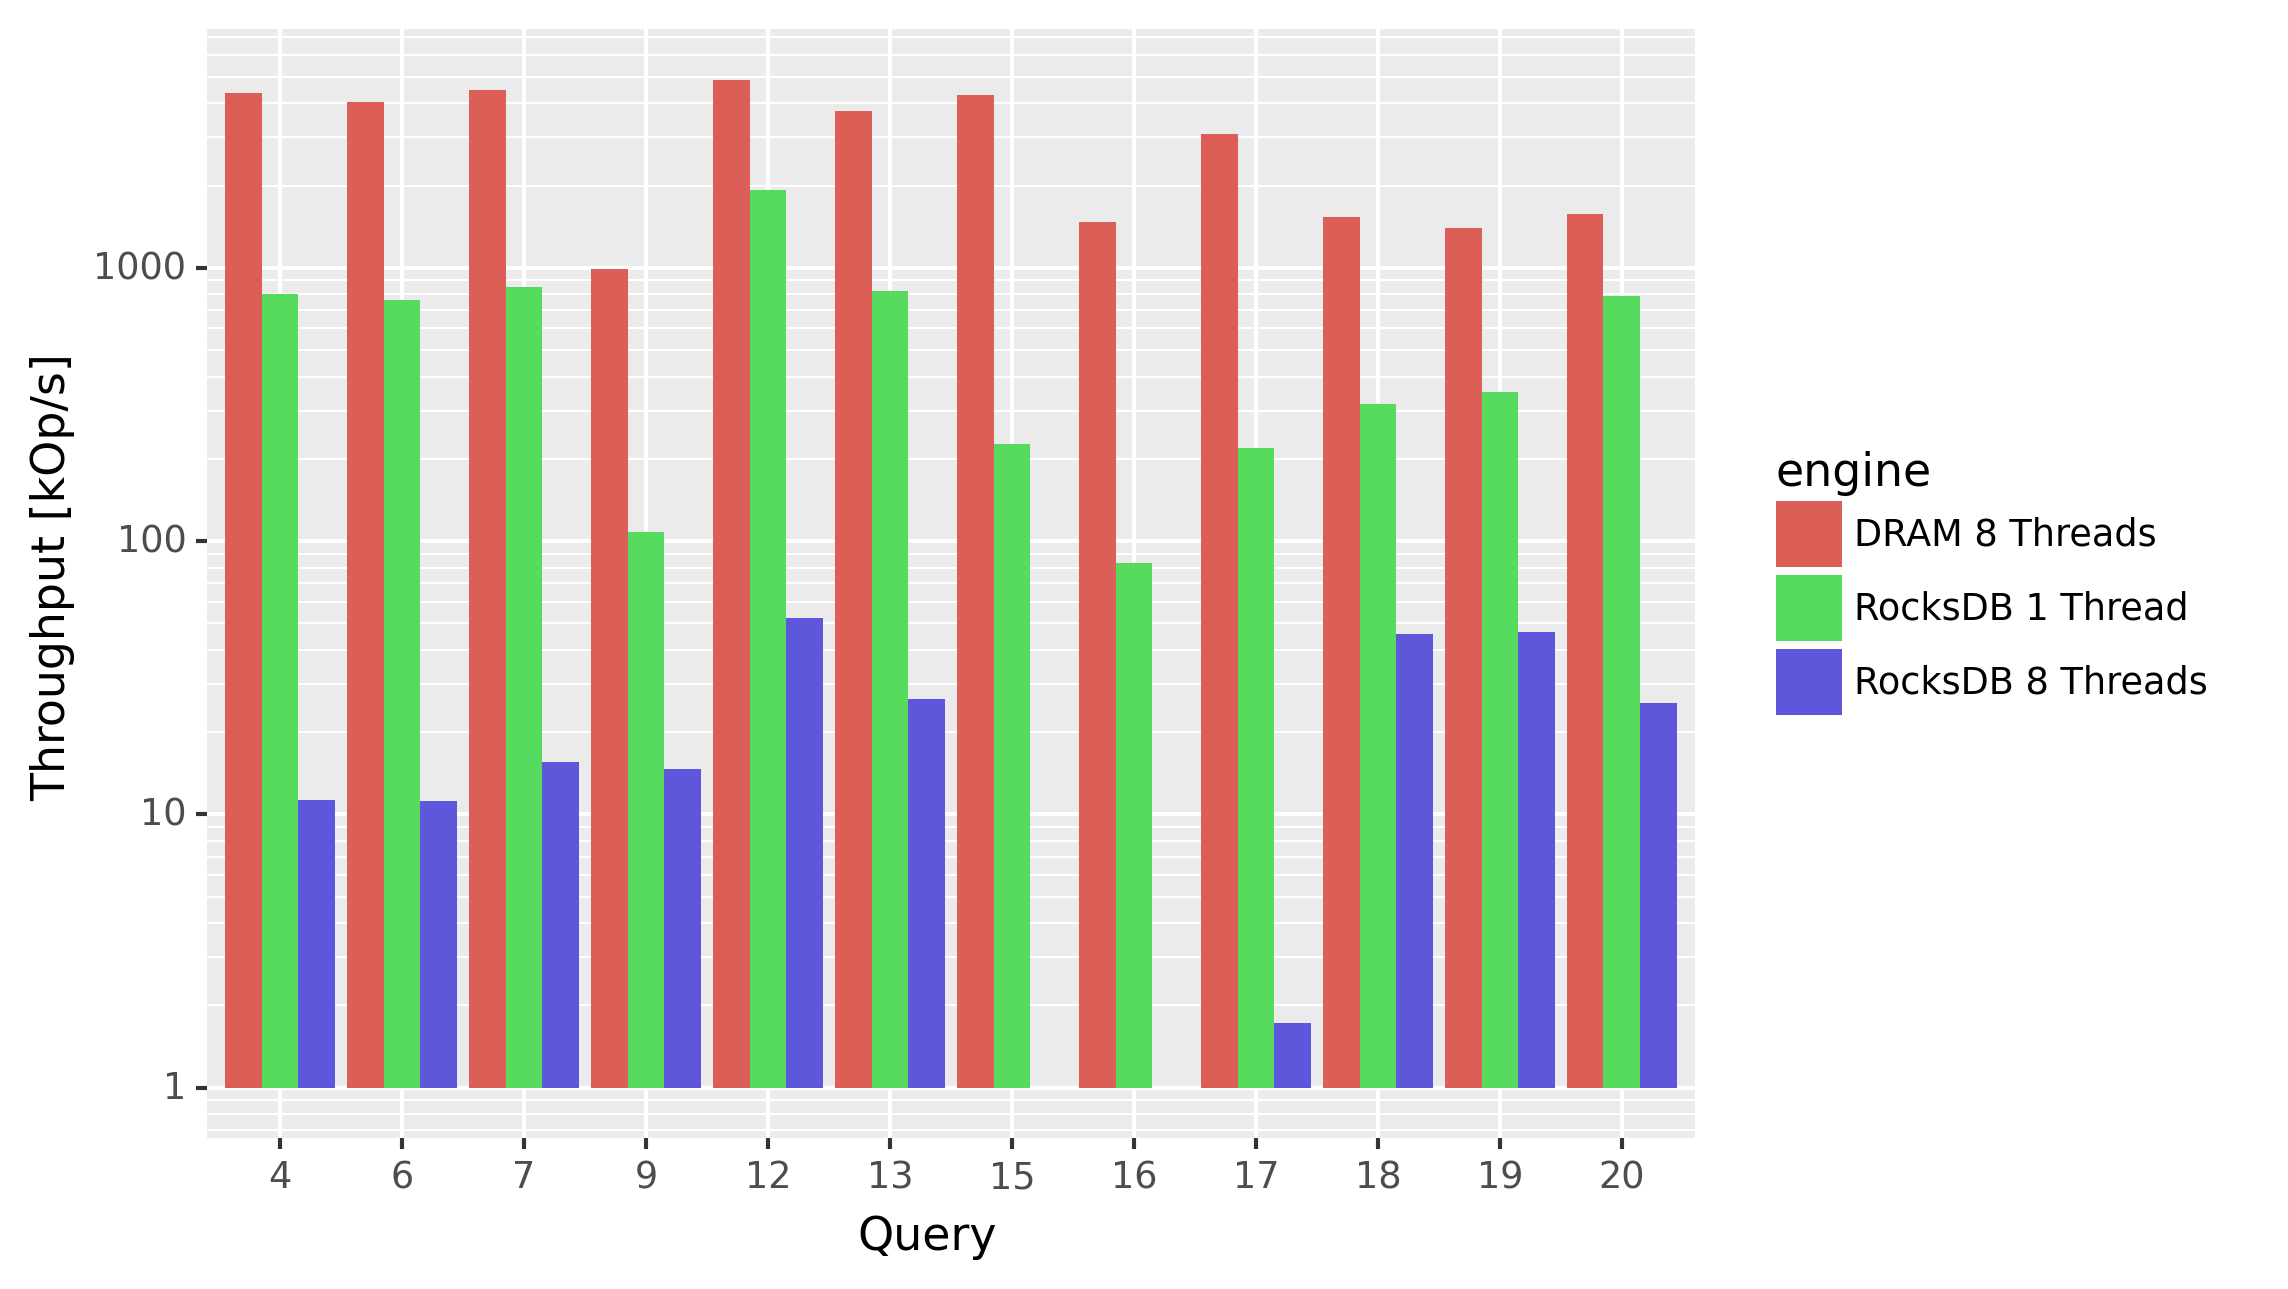
\includegraphics[scale=.43]{graph/rocksdb}
  \caption{Query throughput using RocksDB as a storage layer; higher
    is better.  Note the logarithmic Y axis\label{fig:rocksdb}.}
  \end{center}
\end{figure}

\paragraph{Unable to Leverage Zero-Copy Deserialization.} Besides the
scalability limitations, we also observed significant overheads even
when running on a single thread. This was primarily due to the cost of
deserializing keys and values from RocksDB (which stores data as byte
arrays) into the corresponding Rust types.

\begin{comment}
\paragraph{Overwhelming Configuration Complexity.}

RocksDB offers an overwhelming number of configuration options, making
it nearly impossible for non-experts to ensure optimal settings. The
complexity is so significant that~\cite{thakkar-hotstorage24} resorted
to training a large language model (LLM) to identify good
configurations.

Our attempts did not result in substantial improvements in performance
or scalability. The most effective adjustment was enabling BlobDB,
which increased throughput by approximately 20\%.
\end{comment}

\paragraph{Slow Tests Due to Column Families.} Our core engine is tested
using property-based testing, and therefore runs the same unit-tests
with thousands of different inputs.  When these tests required an
index, RocksDB would quickly generate thousands of short-lived column
families (one for each instantiated test).  This caused our test suite
to slow down significantly, extending the total run time from around 2
minutes to approximately 30 minutes.  We traced this issue to a known
performance degradation in RocksDB when creating many column families,
which is unresolved since 2019.

Since we could not find a suitable pre-existing storage system, the
remaining option was to build our own. Building a key-value embedded
database is a substantial endeavor, so we did not make this choice
lightly.

For this purpose, we implemented our own
SStable-like~\cite{chang-tcs08} file format. The traces write each
batch that is large enough to an individual file.  Batches are always
created in sorted order, which allowed us to write these files
sequentially without any seeks and with minimal in-memory buffering.
Because batches are never modified in-place, the file format and the
code that implements it does not need to make allowances for adding,
removing, or modifying data.

Moreover, the implementation of storage extends the in-memory
shared-nothing architecture: each worker thread processes an
independent stream of data, so the storage layer can be per-thread as
well.

\subsubsection{Checkpointing and fault-tolerance}

The state in delay $\zm$ operators is the only piece of information
that needs to be persisted, checkpointed, or migrated to make \dbsp
computations fault-tolerant.  Since \dbsp circuits operate
synchronously in steps, by checkpointing the state between two
execution steps one obtains a consistent snapshot of the circuit's
state.  There is no need for a complicated synchronization protocol.
Since the index data structures are immutable, taking a snapshot can
be done atomically using copy-on-write.  To complete a checkpoint we
just need to ensure that each snapshot is written on secondary
storage.

\subsection{Compiling SQL to \dbsp}

\begin{figure}[t]
  \begin{center}
    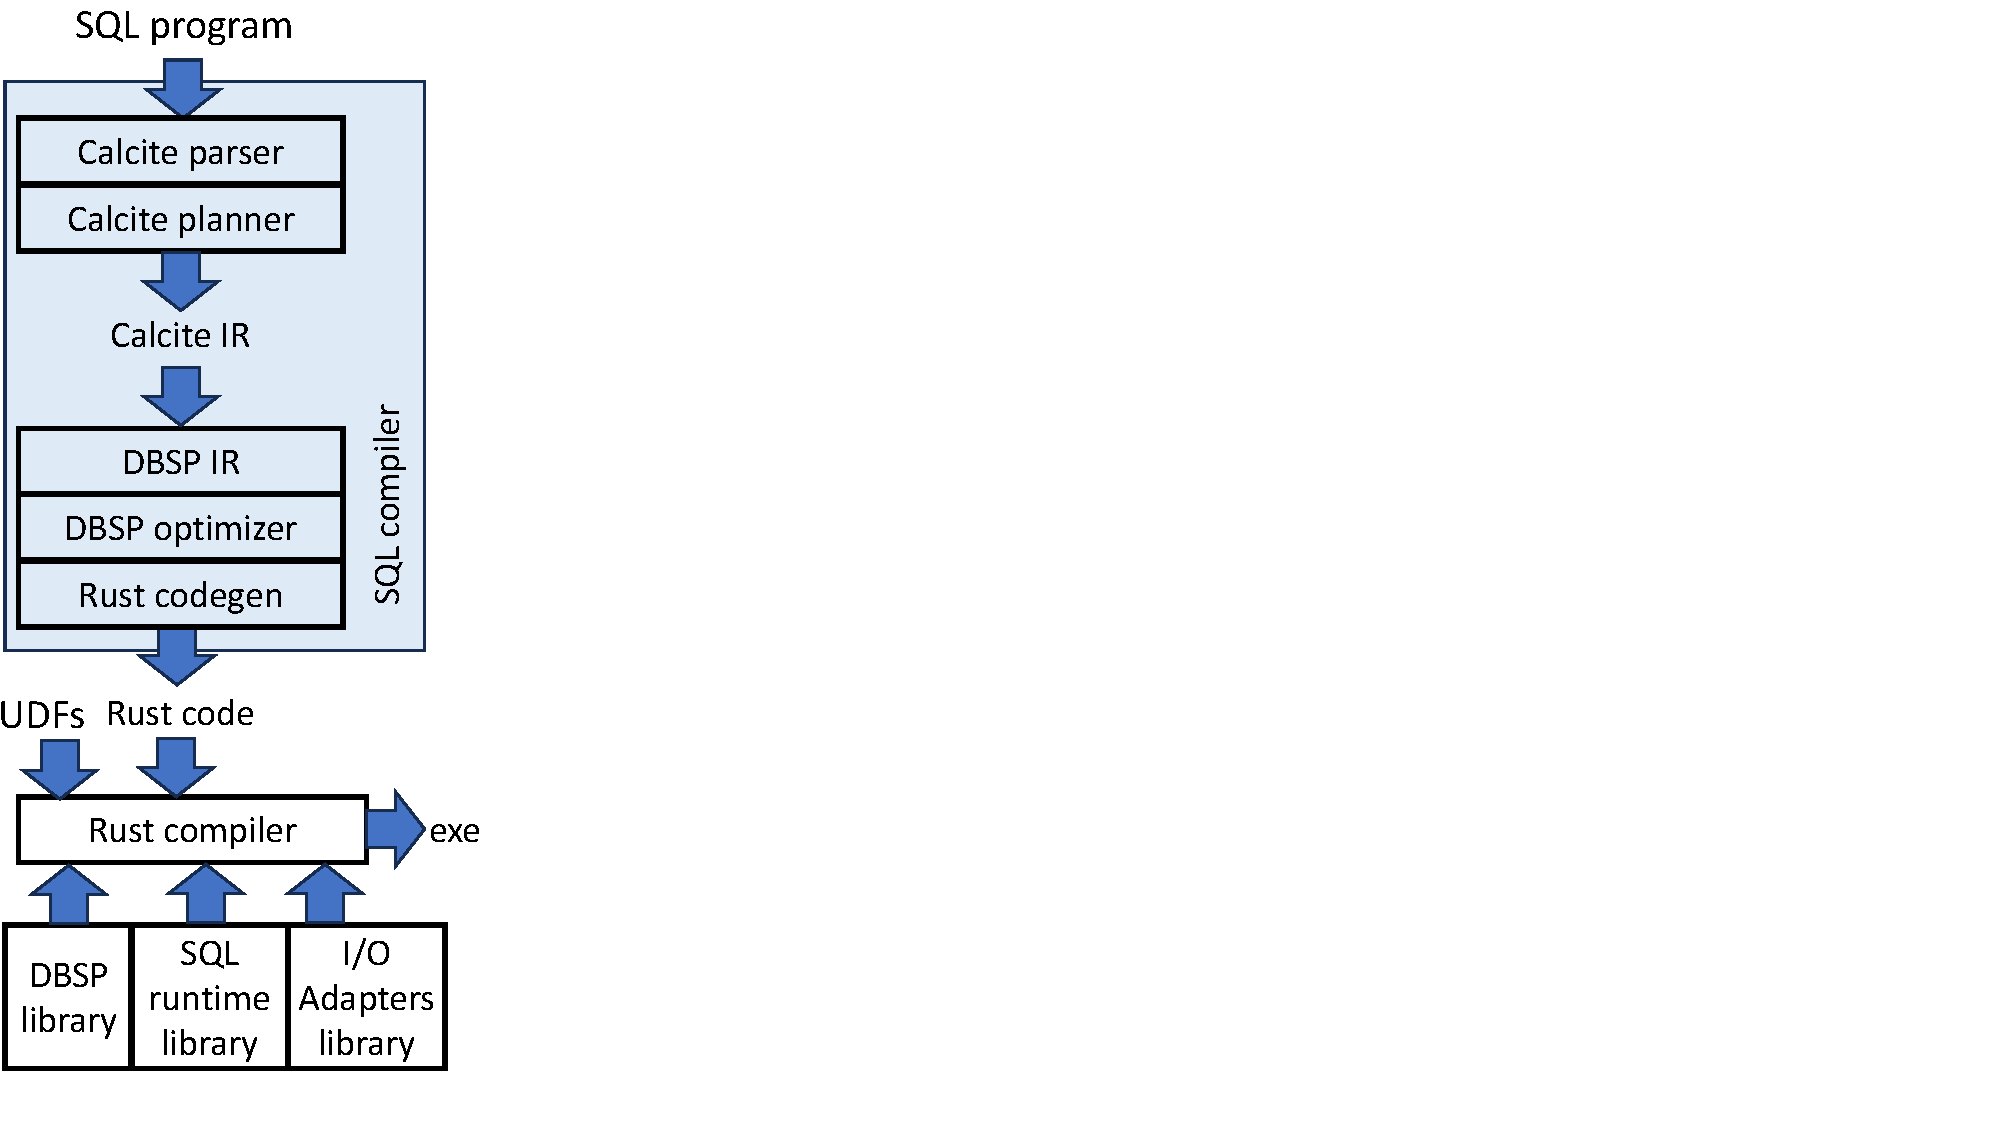
\includegraphics[trim={0 0in 10in 0},clip,scale=.45]{tools.pdf}
    \caption{\label{fig:tools}Architecture of the SQL compiler.}
  \end{center}
\end{figure}

We have built a compiler that accepts SQL programs and generates Rust
programs targeting the \dbsp library.  The architecture of the
compiler is shown in Figure~\ref{fig:tools}.  The implementation
follows Algorithm~\ref{algorithm-inc} very closely.  The input of the
algorithm is a non-incremental query plan, produced by a query
planner.  The algorithm produces an incremental plan that is
``similar'' to the input plan.

The compiler front-end, including the parser, validator, and the plan
generator, are based on the Apache Calcite~\cite{begoli-icmd18}
infrastructure.  Because the incrementalization algorithm starts from
a standard, non-incremental query plan, it can reuse in principle any
existing planner.  We rely on Calcite to decorrelate queries into
joins, for optimizing join ordering and performing a host of
traditional optimizations.

A relational algebra query can be implemented by multiple plans, each
with a different data-dependent cost.  Standard query planners use
cost-based heuristics and data statistics to optimize plans.  A
generic IVM planner many not have this luxury, since the plan
sometimes must be generated \emph{before} (most) data has been fed
to the query.  Nevertheless, all standard query optimization
techniques, perhaps based on historical statistics, can be used to
generate the initial query plan.

The compiler can compile any number of views; each view can depend on
any number of tables or other views.  Given a query $Q$, the compiler
can generate both incremental and non-incremental circuits ($Q$ and
$\inc{Q}$).  The non-incremental circuits are used for validating the
compiler, because they must have the same semantics as a standard
ad-hoc SQL query.

The compiler supports ``standard'' SQL and is mature enough to pass
5+ million SQL Logic Tests~\cite{sqllogictest}.
\begin{itemize}
\item \textbf{types:} \code{NULL}s using the standard SQL ternary
  logic, all standard SQL datatypes (including
  \code{DATE}/\code{TIME}/\\\code{TIMESTAMP}), structured and
  semi-structured types, such as arrays, maps, JSON, multisets,
  \code{UUID}, user-defined types.
\item \textbf{operators:} \code{SELECT}, \code{WHERE}, \code{FILTER},
  \code{HAVING}, \code{ORDER} \code{BY}, \code{LIMIT},
  \code{DISTINCT}, \code{EXCEPT}, \code{INTERSECT}, \code{UNION},
  \code{GROUP BY}, aggregation, inner and outer \code{JOIN}s,
  \code{PIVOT}, \code{ROLLUP}, \code{CUBE}, temporal \code{ASOF JOIN},
  windows \\ (\code{PARTITION BY ... OVER}), \code{UNNEST}, table
  functions, common table expressions, correlated subqueries, and some
  streaming extensions, like tumbling and hopping windows, etc.
\item A large assortment of SQL functions, including user-defined
  functions that can be written in either SQL or Rust.
\item Currently, mutually recursive views support all query operators
  except \code{OVER}.  They are incrementally evaluated using
  Algorithm~\ref{algorithm-rec}.
\end{itemize}

SQL has many constructs that may cause runtime exceptions, such as
arithmetic overflows; in a traditional ad-hoc query system these
would surface as queries that terminate with an error.  Currently
these would also cause a running pipeline to fail completely, but this
solution is unacceptable for a platform for long-running computations.
We are exploring alternative solutions, where a runtime crash would
block the pipeline, giving a chance to the operators to remove
incorrect input data that causes issues.

\subsection{Interacting with the outside world}

\begin{figure}[h]
  \begin{center}
  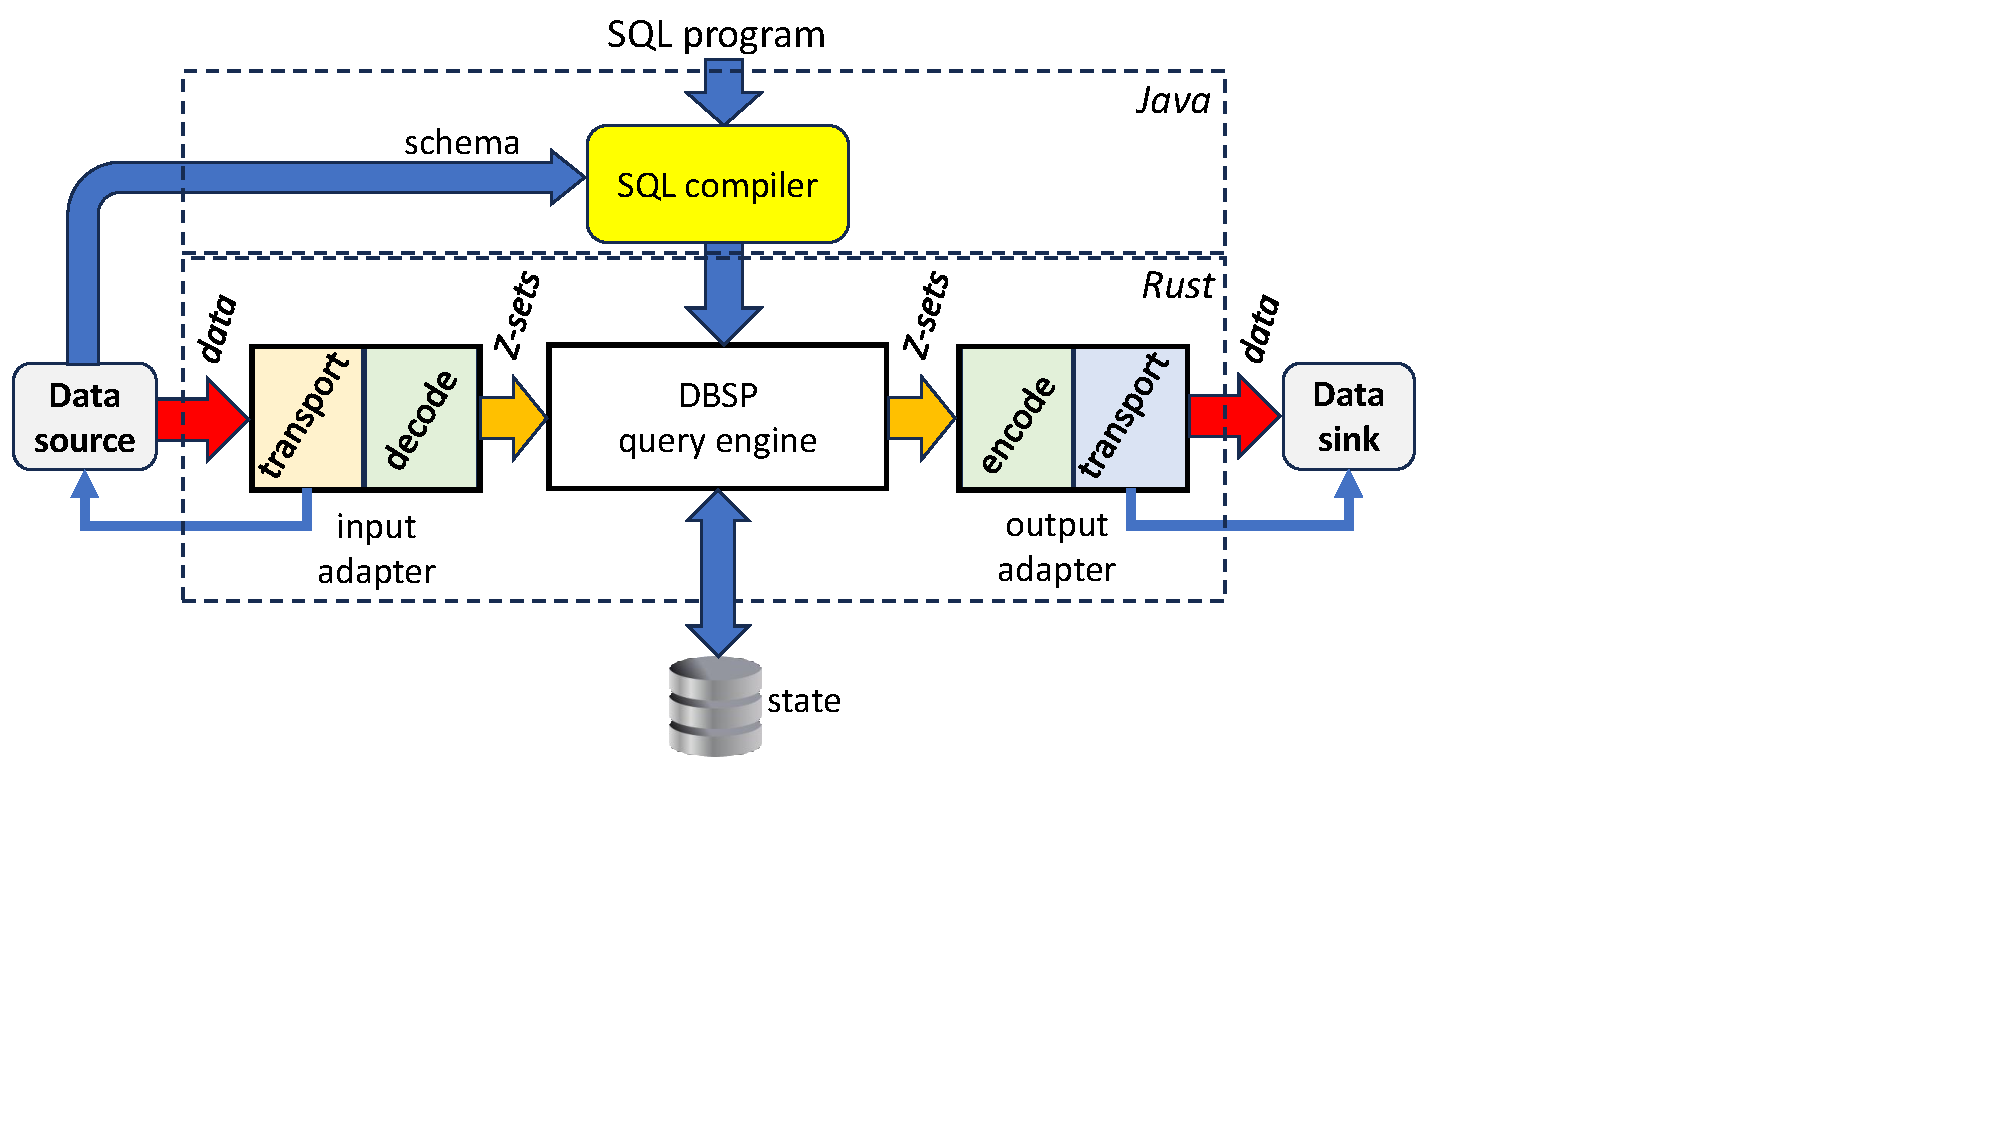
\includegraphics[trim={0 2.2inin 3.7in 0},clip,scale=.33]{adapters.pdf}
  \caption{\label{fig:adapters}Communicating with external data
    sources and sinks.}
  \end{center}
\end{figure}

As noticed many years ago~\cite{labio-vldb00}, database systems are
not designed to interact well with external IVM systems.  We provide a
variety of adapters for interacting with external data sources, both
as inputs and outputs (e.g., Kafka~\cite{kreps-netdb11}, Amazon
S3~\cite{palankar-dadc08}, Google Pub/Sub~\cite{pubsub},
DataFrames~\cite{pandas12}, Delta Lake~\cite{armbrust-vldb20},
database CDC streams via Debezium~\cite{debezium}, HTTP, etc., with
more added every day), and using many data formats (CSV, JSON, Arrow,
Avro, Parquet, etc.).  Figure~\ref{fig:adapters} shows how a circuit
uses adapters to communicate with the outside world.  The input
adapters receive data from external sources, buffer it, convert it
into \zrs, and feed it to the circuits.  The output adapters receive
data from the circuit outputs in the form of \zrs, and send it to a
downstream consumer in a suitable format.

\begin{figure}[h]
  \begin{center}
  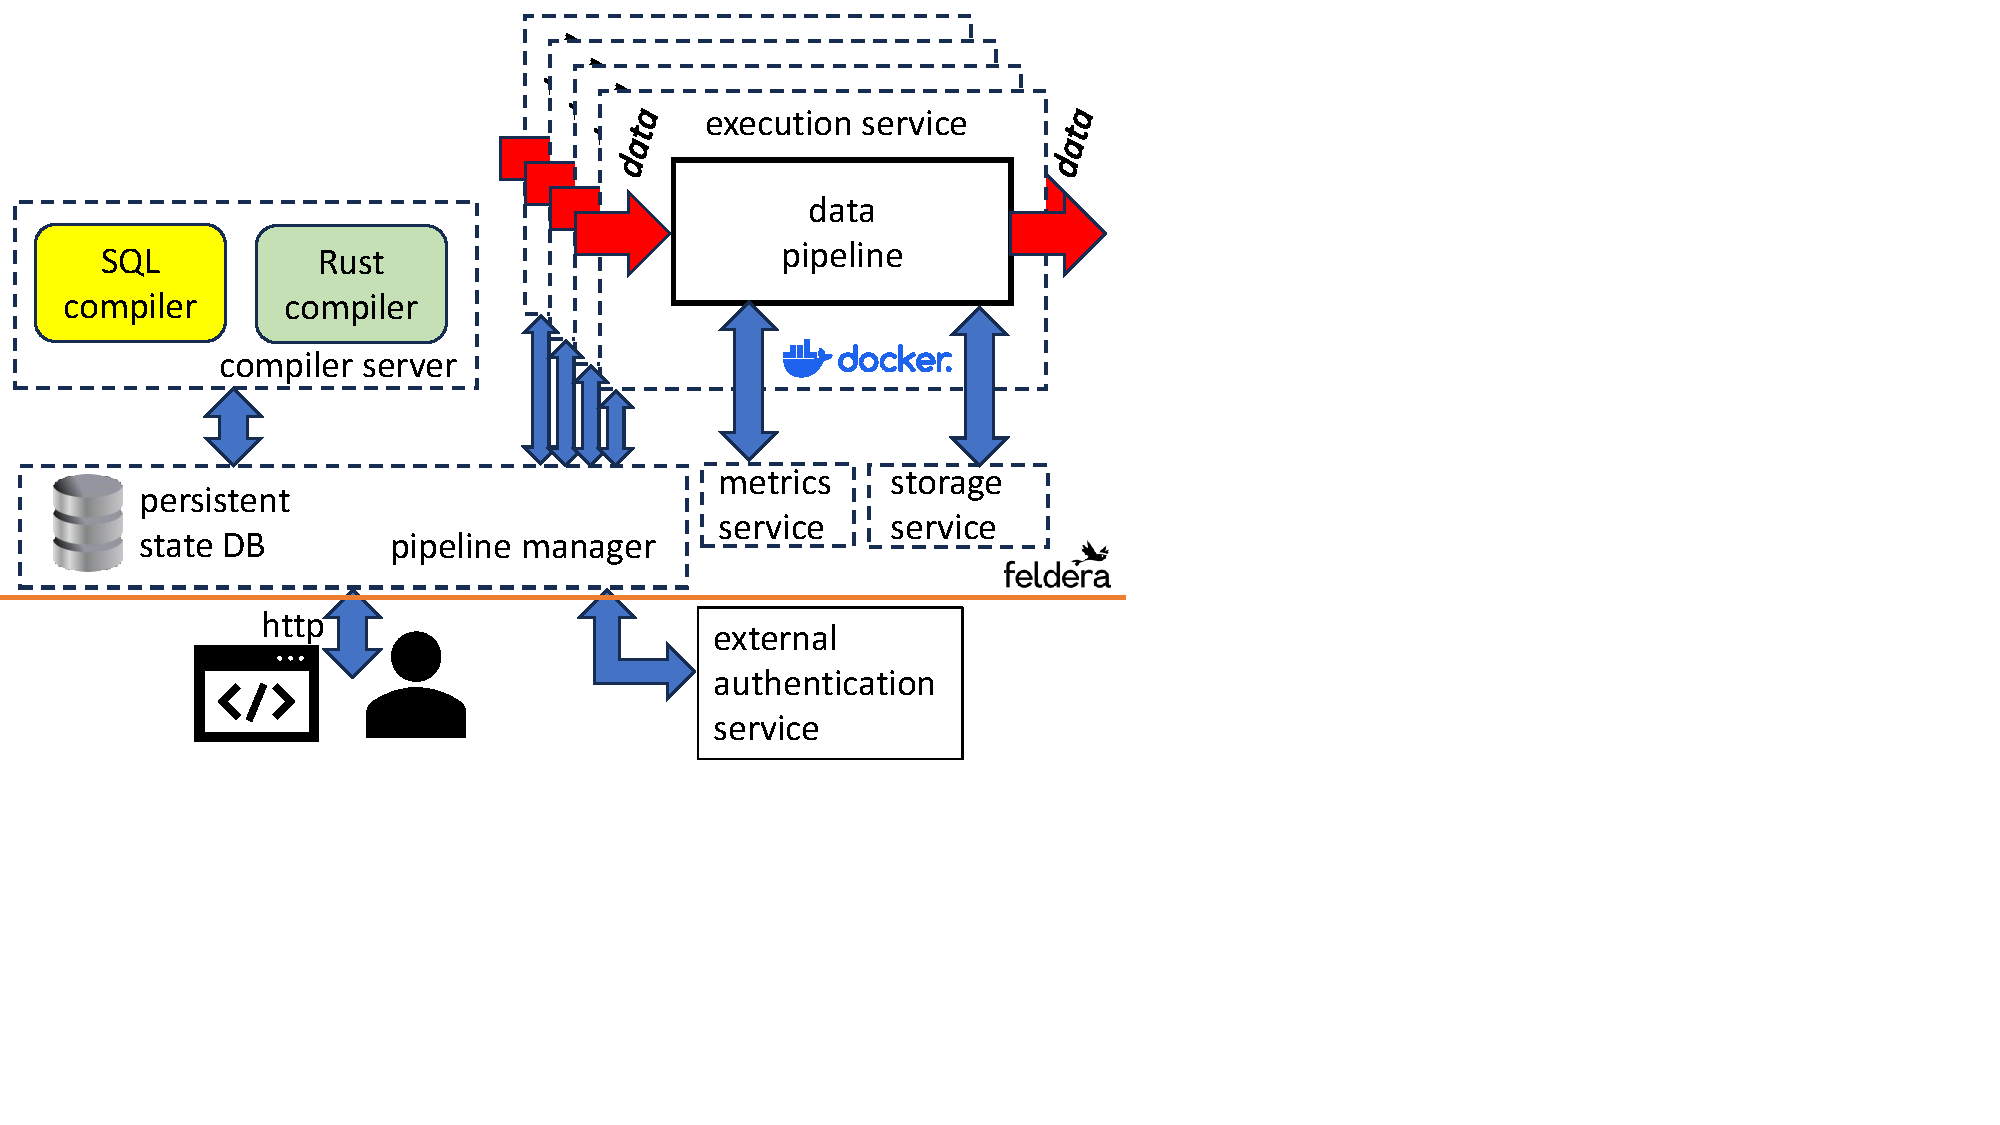
\includegraphics[trim={0 2.4in 4.3in 0},clip,scale=.44]{services.pdf}
  \caption{\label{fig:service}Feldera Service architecture.}
  \end{center}
\end{figure}

\url{Feldera.com} is a start-up that builds a series of software
products around the \dbsp infrastructure.  One of the products is
IVM-as-a-service.  A version of the service-oriented architecture of
the company's cloud offering is shown in Figure~\ref{fig:service}.
The pipeline manager is the centralized control plane, which is
responsible for managing the entire life-cycle of the IVM programs.
These programs are deployed as \emph{pipelines} that run in isolated
Docker containers.  Feldera also offers a cloud form factor, which
distributes the pipeline manager across several communicating services
and uses Kubernetes to run the pipelines.

